%==============================================================================%
\section{Data pipeline} \label{section:pipeline}
%==============================================================================%

The last part of the converting the Wi-Fi probe requests in to footfall was to devise a processing pipeline which combines the 'toolkit' and the methods together.
Figure \ref{figure:processing:pipeline:full} shows the pipeline.
essentially three steps preprocessing where the data is changed and modified for management.
Processing where it is converted to estimated footfall. 
Post processing where theis estimate is adjusted to better reflect the real world.

\begin{figure*}
  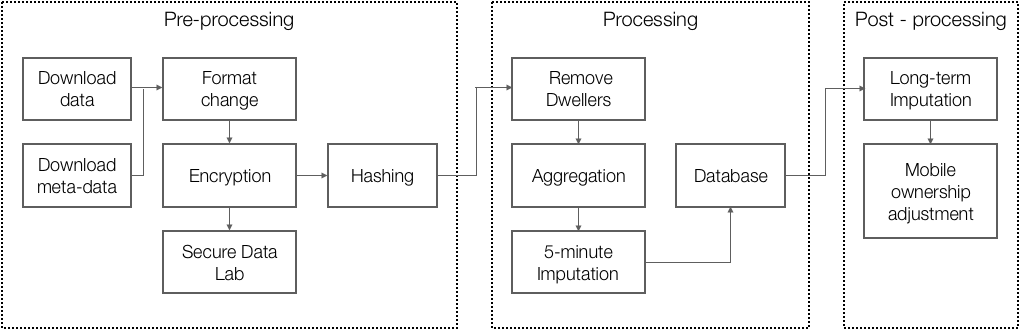
\includegraphics[trim={0 0 0 0},clip]{images/processing-pipeline-full.png}
  \caption{The complete data processing pipeline which takes in raw probe requests from Smart Street Sensor project and outputs footfall estimations.}
  \label{figure:processing:pipeline:full}
\end{figure*}

%------------------------------------------------------------------------------%
\subsection{Pre-processing}
%------------------------------------------------------------------------------%
Pre processing aims are to convert the data into a format which can be used for processing.
It also includes securing the personal part of the data.
hashing where MAC addresses are converted into secure hashes.
the salt was rotated every week to dissuade timing attacks for de-anonymisation.
finally encrypting the non-hashed data and transfer it to the lab using physical media. 
results in csvs which don't have any personal information.

%------------------------------------------------------------------------------%
\subsection{Processing}
%------------------------------------------------------------------------------%
Processing involves the methods discussed in Section \ref{section:processing}.
separated into global and local.
in global.
Probe requests were aggregated based on the MAC addresses for every 5 minute interval to remove short term dwellers.
Probes with repeating MAC addresses in 30 minutes were removed to remove long term dwellers.
Resulting in ambient mobile device estimation around the sensor.
probes to device ration was calculated for each interval and used to calculate devices generating local probes.
The sum of these gives us the estimated number of phones and hence people around the area.
removed noise from devices and long dwellers.
gaps less than 15 minutes are filled using spline based method. Kalman filter.


%------------------------------------------------------------------------------%
\subsection{Post-processing}
%------------------------------------------------------------------------------%
Post processing takes this estimated people and adjusts it to match the real-world.
for footfall, the counts were adjusted with an adjustment factor.
adjustment factor calculated using manual survey for short periods of time and looking at ambient population estimate at that time.
this also removes error caused due to mobile ownership in short term.
The long term trend is offset using 0.2\% per week for offsetting the long term growth in the mobile device ownership.
Finally long term gaps are filled using aseasonally decomposed method for long term

%------------------------------------------------------------------------------%
\subsection{Conclusions}
%------------------------------------------------------------------------------%
Results in cleaned counts, which does not have the uncertainties
it doesn't have problems while doing more research on them.

%------------------------------------------------------------------------------%
